\section[Problemstellung]{Datenassimilation}
\begin{frame}[<+->]
\frametitle{Datenssimilation}
    \begin{block}{Problem}
    \begin{itemize}
     \item $\dot{x} = F(x),~ x_0 = c,~F\text{ Lipschitz}$ 
     \item $x_{obs}$ \quad - \quad Observierungsparameter
    \end{itemize}

    \end{block}
   \begin{block}{Plot}
      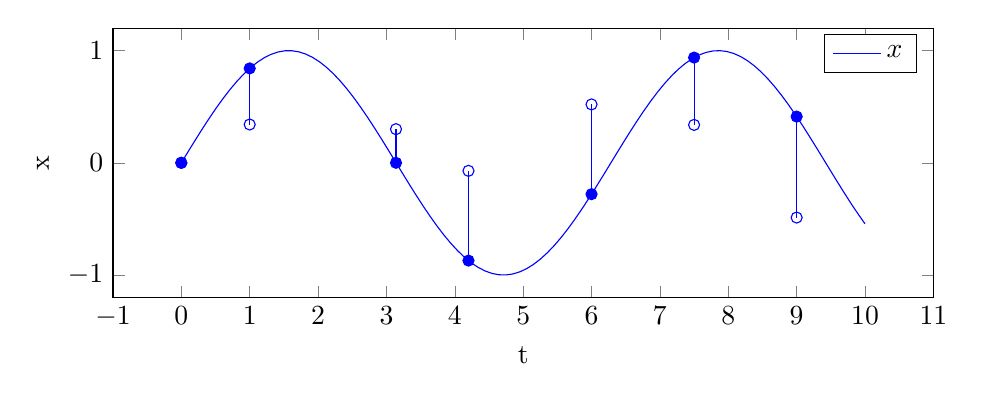
\begin{tikzpicture}
     \begin{axis}[width=12cm,height=5cm,xlabel=t,ylabel=x] 
     \addplot[blue,domain=0:10,samples=100]{sin(deg(x))};
     \addplot+[blue,draw=none,mark=*, mark options={blue},error bars/.cd, y dir=plus,y explicit,error mark=o,error mark options={blue,mark size=2pt}] 
     coordinates { 
      (0,0) +- (0,0) 
     (1,0.8415) +- (0.5,-0.5) 
     (3.14,0) +- (0.05,0.3) 
     (4.2,-0.8715) +- (0,0.8)
     (6.0,-0.27942) +- (0,0.8)
     (7.5,0.93799) +- (0.1,-0.6) 
     (9,0.41212) +- (0.3,-0.9)}; 
    
  \legend{$x$}
     \end{axis}
   \end{tikzpicture}
  %\begin{tikzpicture}
    %\begin{axis}[width=12cm,height=5cm,xlabel=t,ylabel=x] 
    %\addplot[blue,domain=0:10,samples=5]{2/pi/55*asin(sin(deg(x)))};
     %\addplot+[blue,draw=none,mark=*, mark options={blue},error bars/.cd, y dir=plus,y explicit,error mark=o,error mark options={blue,mark size=2pt}] 
    %coordinates { 
    %(1,0.18) +- (0.5,-0.5) 
    %(3.14,0.1) +- (0.05,0.2) 
    %(4.2,-0.45) +- (0,0.5)
    %(7.5,0.8) +- (0.1,-0.6) 
    %(9,0.1) +- (0.3,-0.9)}; 
    %\legend{$x$}
    %\end{axis} 
  %\end{tikzpicture}
   \end{block}


\end{frame}
\begin{frame}[<+->]
  \frametitle{Convergence $\frac{\partial J(x_0)}{\partial x_0}$ }
	\begin{block}{Aim: Minimize cost function}
	\[
		\min_{x_o} J(x_0) = \frac{1}{2}\int_0^T \|x - x_{Obs}\|^2dt
	\]
	\end{block}
	\begin{block}{Solution steps}
	\begin{flushright}
	
	\end{flushright}
	
	\begin{enumerate}
	 \item Calculate cost function J
	 \item Calculate $\frac{\partial J(x_0)}{\partial x_0}$ via adjoint model
	 \item Solve mathematical program e.g. with linesearch methods
	\end{enumerate}
	\end{block}
\end{frame}
 
\begin{frame}[<+->]
  \frametitle{Convergence $\frac{\partial J(x_0)}{\partial x_0}$ }
  \begin{figure}
  \centering
%   \animategraphics[loop,height=5cm]{24}{Bilder/animation/animation_}{0}{118}
  \end{figure}
\end{frame} 